\section{Introduction to Control}

\subsection{Open Loop Control}
(åbensløjfe regulering)

\begin{center}
	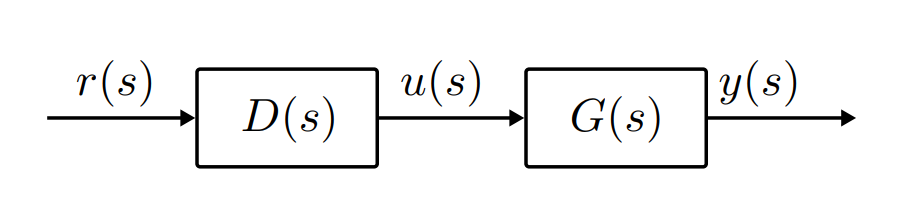
\includegraphics[width=0.6\textwidth]{Images/openLoopControl.png}
\end{center}


Steady-State Value of Time Function:

Suppose that Y(s) is the Laplace transform of y(t). Then the final value of y(t) is either:
\begin{itemize}
	\item{Ubounded. If Y(s) has any poles in the open right half-plane (unstable)}
	\item{Undefined. If Y(s) has a pole pair on the imaginary axis.}
	\item{Constant. If all poles of Y(s) are in the open left half-plane, except for one at s=0}
\end{itemize}

\textbf{The Final Value Theorem (slutværdi-sætningen)}

If all poles of sY(s) are in the open left half-plane, then:
$$\lim_{t \to \infty} y(t) = \lim_{s \to 0} sY(s)$$

The Final Value Theorem determines the constant value that the impulse response of a stable system converges to.
The theorem can also be used to determine the DC gain of a system, i.e., the output when a step input is applied to the system.

By integrating an impulse response, the step response is obtained. The step response is the integral of the impulse response,
and the impulse response is the derivative of the step response.

If the system has a disturbance an open loop control system will not be able to compensate for this.

\subsection{Feedback Control}
(tilbagekobling). Tilbagekobling anvendes for at elminere forstyrrelsesundertrykkelse.

The connection of a controller K(s) and a system (also called plant) G(s) is called a closed-loop system.
\begin{center}
	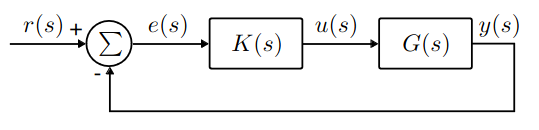
\includegraphics[width=0.6\textwidth]{Images/feedbackControl.png}
\end{center}

e(s) is the error signal, and is the difference between the reference signal r(t) and the output signal y(t).
The error signal is used to adjust the input signal u(t) to the system. The controller K(s) is used to adjust the input signal.

The closed-loop transfer function is given by:
$$\frac{y(s)}{r(s)} = \frac{G(s)K(s)}{1+G(s)K(s)}$$

K(s) can be designed to meet certain requirements, such as stability, disturbance rejection, and sensitivity analysis.


\textbf{Stability}

The closed-loop system is stable if all the closed-loop poles are in the
open left half-plane.

The \textbf{loop gain (sløjfe-forstærkning)} is defined as: $L(s) = G(s)K(s)$.
The closed-loop poles are given by:
$$1+L(s) = 0$$

The closed loop poles satisfy:
$$1+L(s) = 0 \Rightarrow L(s) = -1$$

\textbf{Disturbance Rejection}

Open loop control system:
\begin{center}
	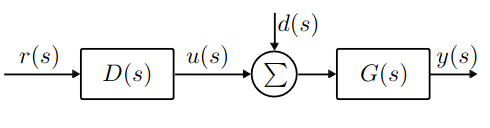
\includegraphics[width=0.6\textwidth]{Images/openLoop.png}
\end{center}
The output is given by:
$$y_m(s)=G(s)d(s)+G(s)D(s)r(s)$$


Closed loop control system:
\begin{center}
	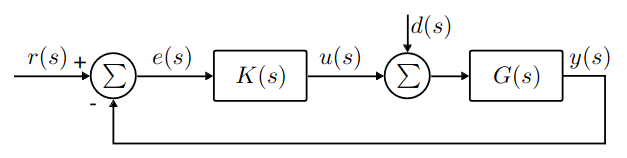
\includegraphics[width=0.6\textwidth]{Images/closedLoop.png}
\end{center}
The output is given by (superposition can be applied for deriving the expression):
$$y_m(s) = \frac{G(s)}{1+G(s)K(s)}d(s) + \frac{G(s)K(s)}{1+G(s)K(s)}r(s)$$

The larger the amplification of the feedback loop, the smaller the effect of the
disturbance on the output.

%Muligvis slide 16 her

\textbf{Sensitivity Analysis}

The sensitivity S of the open-loop system is given by the ratio of $\delta T_{ol}/T_ol$ to $\delta G_0/G_0$.
For the open loop system S=1. $\delta$ is the relative change in the transfer function.

For the closed loop the sensitivity is given by:
$$S = \frac{1}{1+G_0 K_0}$$
This means that a large amplification leads to a low sensitivity.

\textbf{Linearization}
Taylor approximation, YES.


\subsection{Steady State Tracking}

\textbf{Definition of system type}

Stable systems can be classified according to its system type, defined to be the
degree of the polynomial
for which the steady-state error in a nonzero finite constant.


\begin{center}
	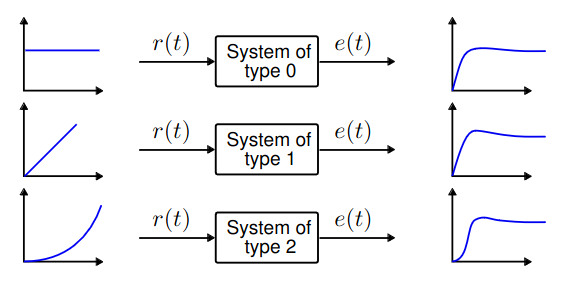
\includegraphics[width=0.6\textwidth]{Images/systemTypes.png}
\end{center}


An expression for the tracing error is computed to determine the steady-state error. The error is given by:
$$e(s) = \frac{1}{1+L(s)}r(s)$$
Where r(s) is the reference signal and L(s) is the loop gain.

\textbf{The amount of poles at s=0 in the denominator of L(s) determines the system type.}

Final value theorem is used to determine the steady-state error when
the reference signal is a polynomial $r(t) = t^k 1(t)$.

$$e_ss = \lim_{t \to \infty} e(t) = \lim_{s \to 0} e(s)s$$
$$\lim_{s \to 0} e(s)s = \lim_{s \to 0} s\frac{1}{1+L(s)}r(s)$$
$$\lim_{s \to 0} s\frac{1}{1+L(s)}\frac{1}{s^{k+1}}$$

\subsection{Cascade Control}
A cascade control uses the output from one controller as the input to another controller.


\begin{center}
	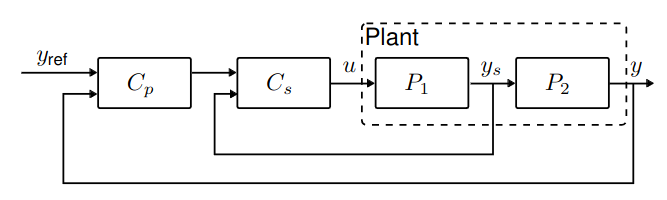
\includegraphics[width=0.6\textwidth]{Images/cascade.png}
\end{center}

The nested control loops are called the inner loop (secondary) and the outer loop (primary).
A fundamental reason for applying cascade control is to obtain better disturbance rejection
and lower sensitivity to parameter variations.


\subsection{DC Motor Dynamics}



\subsection{Examples}
